% CVPR 2024 Paper Template; see https://github.com/cvpr-org/author-kit

\documentclass[10pt,twocolumn,letterpaper]{article}

\usepackage{cvpr}      % To produce the REVIEW version
% \usepackage[pagenumbers]{cvpr} % To force page numbers, e.g. for an arXiv version

% Import additional packages in the preamble file, before hyperref
%
% --- inline annotations
%
\usepackage[dvipsnames]{xcolor}
\newcommand{\red}[1]{{\color{red}#1}}
\newcommand{\todo}[1]{{\color{red}#1}}
\newcommand{\TODO}[1]{\textbf{\color{red}[TODO: #1]}}
% --- disable by uncommenting  
% \renewcommand{\TODO}[1]{}
% \renewcommand{\todo}[1]{#1}



\definecolor{cvprblue}{rgb}{0.21,0.49,0.74}
\usepackage[pagebackref,breaklinks,colorlinks,citecolor=cvprblue]{hyperref}

\def\paperID{*****} % *** Enter the Paper ID here
\def\confName{CVPR}
\def\confYear{2024}

%%%%%%%%% TITLE - PLEASE UPDATE
\title{Warm Up Exercises 1, 2}

\author{Rishitosh Kumar Singh\\
Arizona State University\\
% Institution1 address\\
{\tt\small rksing18@asu.edu}
}

\begin{document}
\maketitle
\begin{abstract}
    This report is part of the assignment that is due on 21st Jan 2024. This report consists of two practice problems and by completing these problems I got to know how datasets and dataloaders work in Pytorch, and how to train and test a neural network with Pytorch.
\end{abstract}    
\section{Warm Up Exercise 1}
\label{sec:warmup1}
    \subsection{Problem}
        In this exercise, we were provided with two datasets. The objective was to proficiently load the data using PyTorch's dataloaders and dataset APIs, and subsequently, successfully generate matplotlib plots by writing the images.
    \subsection{Solution}
        
    To load the provided dataset, custom PyTorch dataset classes were crafted. These classes offer flexibility to handle datasets of various types and formats. The torchvision.io.read\_image function is employed for reading PNG/JPG images, while the pydicom library is utilized for reading DICOM data.
    
    \subsubsection*{Transformations}
        \begin{figure}[b]
            \begin{subfigure}[t]{\linewidth}
                \centering
                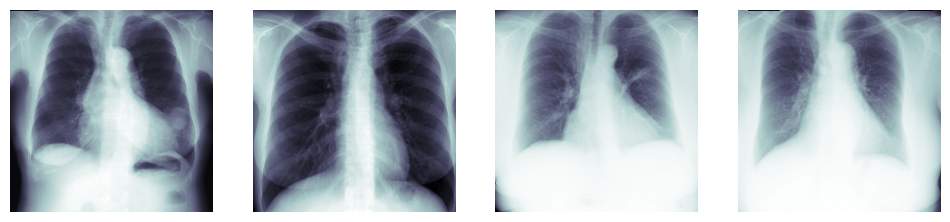
\includegraphics[width=\linewidth]{images/chest-xray-output.png}
                \caption{PNG/JPG dataset}
                \label{fig:png-image}    
            \end{subfigure}
            \begin{subfigure}[t]{\linewidth}
                \centering
                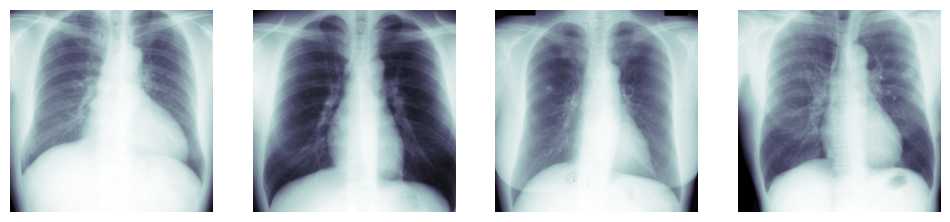
\includegraphics[width=\linewidth]{images/dicom.png}
                \caption{DICOM dataset}
                \label{fig:dicom-image}
            \end{subfigure}
            \caption{XRay images batch}
            \label{fig:xray-images}
        \end{figure}
        \begin{itemize}
            \item When PNG/JPG images were loaded, a resize transformation was applied to change the images to a size of $256$x$256$. \Cref{fig:png-image} displays a batch of 4 images from the PNG/JPG dataset.
            \item After loading DICOM data, a sequence of transformations was employed. At first, the image type is converted from uint16 to uint8, because PyTorch resize function does not support uint16 dtype. Subsequently, the tensor is converted to a PIL image, and the image is resized. Following the dataset loading, all the images are plotted in a matplotlib plot. \Cref{fig:dicom-image} displays a batch of 4 images from the DICOM dataset.
        \end{itemize}
    
\section{Orientation}
\label{sec:warmup2}

    In this introductory practice exercise, chest X-rays were provided, and the task involved training/fine-tuning a model to determine the orientation of these X-rays.

\subsection{Dataset}
    The provided dataset consists of RGB X-ray images with 948 training samples depicting various orientations and an additional 40 samples for testing. All images are of size $128$x$128$ and are oriented either as up (0), right (1), down (2), or left (4). Due to the absence of a dedicated validation set in the given dataset, I have randomly partitioned the training samples into training and validation sets in 8:2 ratio. 
\subsection{Model Used}

    For this task, I utilized ResNet18 as the backbone model with pre-trained weights from ImageNet. Since ResNet18 was originally trained on ImageNet, its output tensor has a size of (n, 1000). However, in the given problem, we are specifically dealing with 4 classes (up, right, down, left). Therefore, I introduced a fully connected layer followed by a log-softmax layer to obtain probabilities for each class. Refer to \Cref{fig:orientation_model} for a graphical representation of the model architecture.
    
    % \begin{figure}[htbp]
    %     \centering
    %     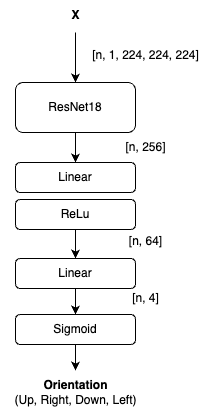
\includegraphics[width=0.4\linewidth]{images/OrientationModel.png}
    %     \caption{Graph of model used}
    %     \label{fig:model_graph}
    % \end{figure}

\subsection{Training}
    
    The model is trained using the categorical cross-entropy loss function with stochastic gradient descent as the optimizer. As the Log-Softmax layer is already included in the model, the torch.nn.NLLLoss function is employed instead of a torch.nn.CrossEntropyLoss. Four experiments were conducted with learning rates of 0.001, 0.003, 0.01, and 0.03, and the results were averaged. Refer to \Cref{fig:learning-curve} for a demonstration of the learning curve from one of the experiments.

    \begin{figure}[htbp]
        \centering
        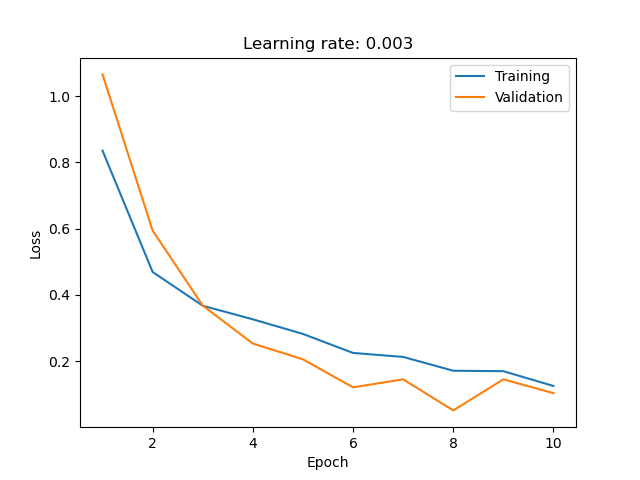
\includegraphics[width=\linewidth]{../plots/orientation/2024-01-20 21:01:42-train-val-plot.png}
        \caption{Learning curve}
        \label{fig:learning-curve}
    \end{figure}

\subsection{Results}

    \begin{figure}[!htbp]
        \centering
        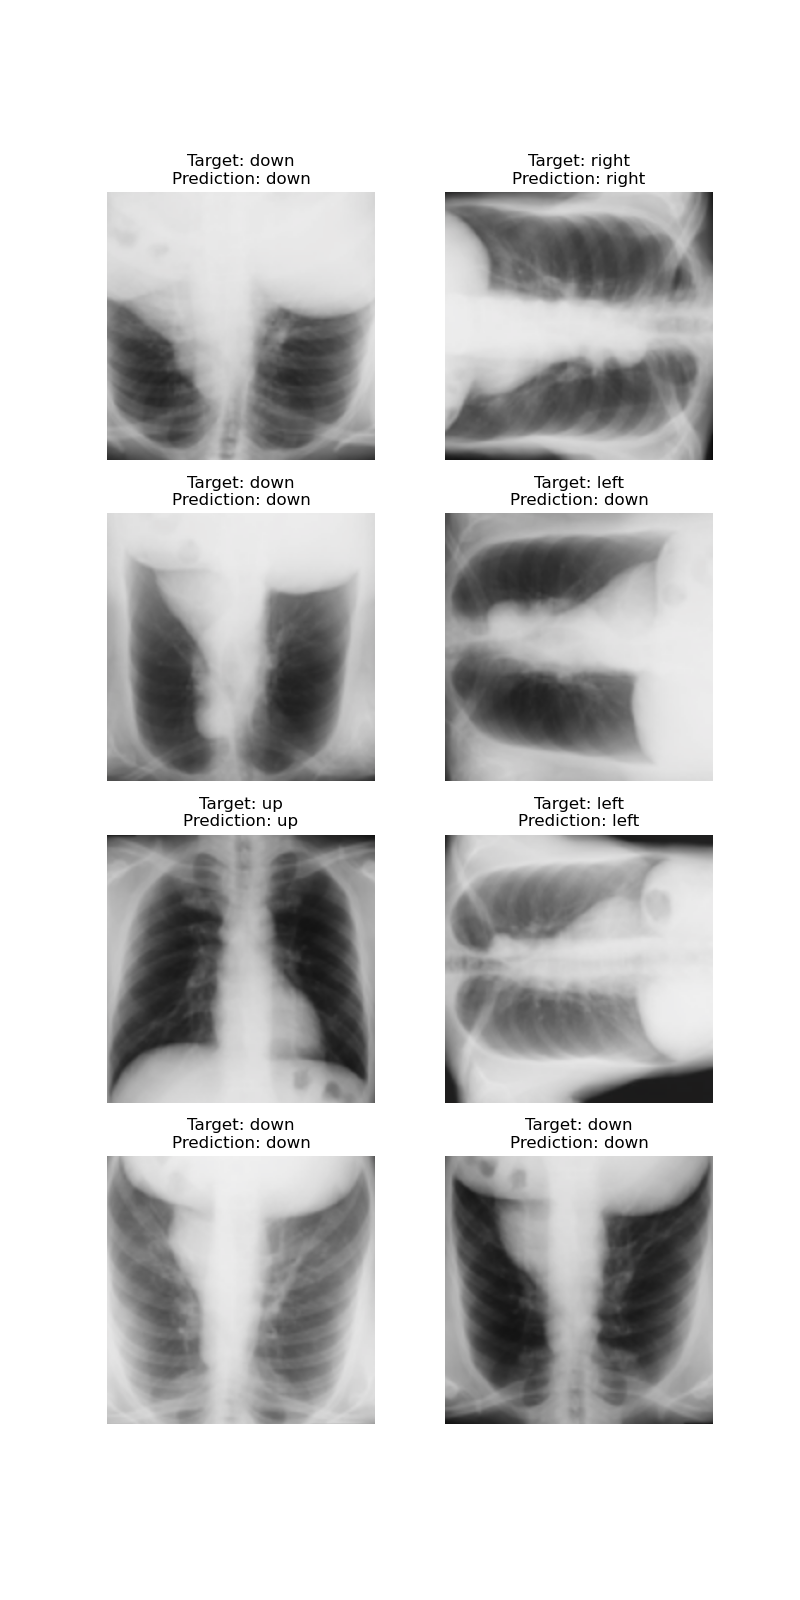
\includegraphics[width=\linewidth]{../plots/orientation/2024-01-20 21:01:42.png}
        \caption{Predictions on few samples of test data}
        \label{fig:results}
    \end{figure} 

    After fine-tuning the model with the ResNet18 backbone network, the model was transitioned to testing and evaluated on the provided test samples. On average, it achieved an accuracy of $96.87\%$, and in some experiments, $100\%$ accuracy was also attained. \Cref{fig:results} showcases some of the test samples along with their model predictions and target classes.

% {
%     \small
%     \bibliographystyle{ieeenat_fullname}
%     \bibliography{main}
% }

% WARNING: do not forget to delete the supplementary pages from your submission 
% \input{sec/X_suppl}

\end{document}
